% !TeX program = lualatex
% !TeX root = baseline_poster.tex
\documentclass[final]{beamer}

% ====================
% Packages
% ====================

\usepackage[T1]{fontenc}
\usepackage{lmodern}
\usepackage[size=custom,width=118.9,height=84.1,scale=1.0]{beamerposter}
\setbeamerfont{block body}{size*={24pt}{26pt}}
\usetheme{gemini}

\usepackage{graphicx}
\usepackage{booktabs}
\usepackage{tikz}
\usepackage{pgfplots}
\pgfplotsset{compat=1.14}
\usepackage{anyfontsize}
\usepackage{tabularx}
\usepackage{makecell}
\usepackage[table]{xcolor}

% ====================
% Lengths
% ====================

% If you have N columns, choose \sepwidth and \colwidth such that
% (N+1)*\sepwidth + N*\colwidth = \paperwidth
\newlength{\sepwidth}
\newlength{\colwidth}
\setlength{\sepwidth}{0.025\paperwidth}
\setlength{\colwidth}{0.3\paperwidth}

\newcommand{\separatorcolumn}{\begin{column}{\sepwidth}\end{column}}

\newcommand{\subtitleformat}[1]{%
  {\fontsize{32pt}{38pt}\selectfont\color{blue!60!black}\textbf{#1}}%
}

\usepackage[backend=biber,style=numeric,sorting=none,maxbibnames=3]{biblatex}
\addbibresource{poster.bib}

% ====================
% Title
% ====================

\title{\fontsize{85}{100}\selectfont \raisebox{-0.2\height}{
\includegraphics[height=100pt]{"images/VeriFi logo.png"}} \hspace{0.5cm} A Verifiable Social Platform for Financial Claims}

\author{Your Name \and Advisor: Advisor Name}

\institute[shortinst]{\inst{1} Boğaziçi University Department of Computer Engineering}

\logoright{
\includegraphics[width=6cm]{logos/boun logo.pdf}}
\logoleft{
\includegraphics[width=6cm]{logos/boun logo.pdf}}

% ====================
% Body
% ====================

\begin{document}

\begin{frame}[t]
\begin{columns}[t]
\separatorcolumn

% ====================
% First Column
% ====================
\begin{column}{\colwidth}

  \begin{block}{What is VeriFi}
    A finance social media app, consisting of claims and suggested positions
    - 
  \end{block}

  \begin{block}{\fontsize{42}{48}\selectfont\bfseries Motivation}
    Don't know which stock to buy? Or whether to buy gold or not in this chaotic environment?\\
    Wanna take some insights from an expert? But who? Who to trust?\\
    Posts in twitter? sketchy technical analysis in TradingView? Telegram groups for investment?
    
    \vspace{1cm}
    These platforms don't supply:
    \begin{itemize}
        \item social,
        \item verifiable,
        \item quantifiable
    \end{itemize}
    
    \vspace{1cm}
    We supply all of these in \textbf{VeriFi}.
  \end{block}


  \begin{block}{\fontsize{42}{48}\selectfont\bfseries Design}
    \subtitleformat{Integrated with live data from APIs}\\
    Every content is signed by users.
    
    \vspace{1cm}
    
    \subtitleformat{Reputation Market Ensures:}
    \begin{itemize}
        \item early foresighters are rewarded more, no copycating
        \item bullshit claims are prevented, claim rationally
        \item trivial claims are not rewarded, only interesting discussions going on
    \end{itemize}
  \end{block}

  \begin{block}{\fontsize{42}{48}\selectfont\bfseries Components}
    \textbf{Claims, Positions, Reputation Score, Reputation Market, Channels, Proofs}
    
    \vspace{1cm}
    
    \subtitleformat{Reputation Score:}
    \begin{itemize}
        \item how are scores collected?
    \end{itemize}
    
    \vspace{1cm}
    
    \subtitleformat{Why Need Proofs?}
    \begin{itemize}
        \item bypass gdpr
        \item ensure verification
    \end{itemize}
  \end{block}

\end{column}

\separatorcolumn

% ====================
% Second Column
% ====================

\begin{column}{\colwidth}

  \begin{block}{Lifecyle of a Claim in VeriFi}
    
  
  \begin{figure}
    \centering
    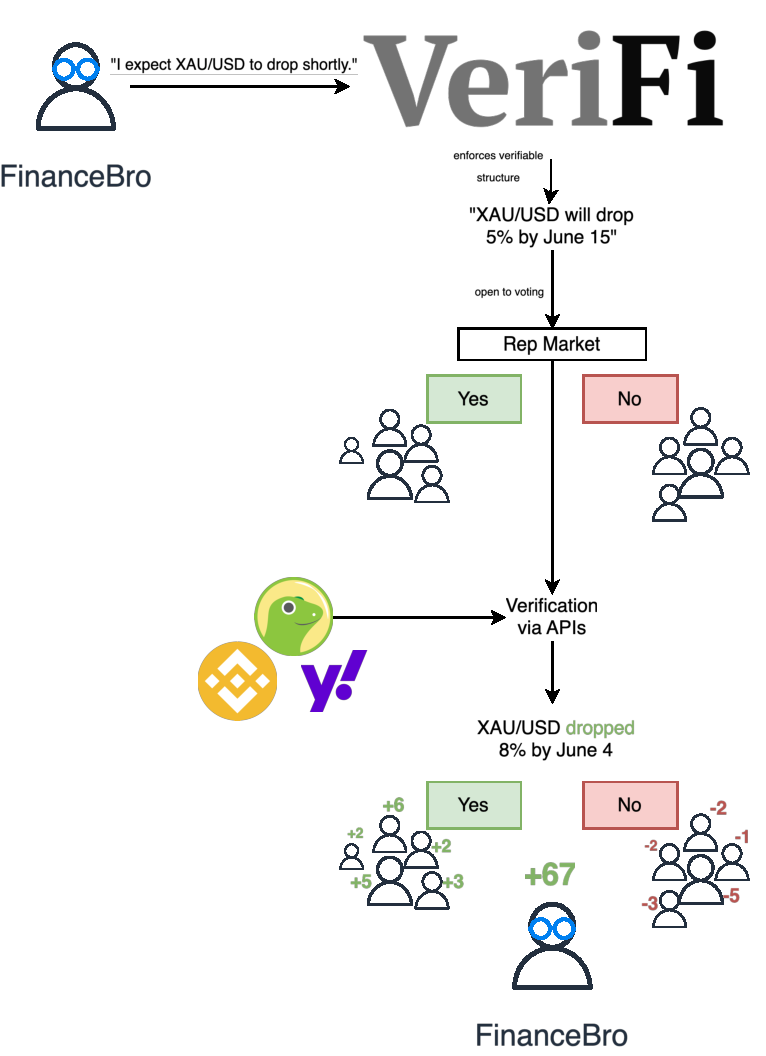
\includegraphics[width=\linewidth]{images/verifi_flow.pdf}
  \end{figure}
  \end{block}

\end{column}

\separatorcolumn

% ====================
% Third Column
% ====================
\begin{column}{\colwidth}

\begin{block}{How Reputation Market Work}
  
\end{block}


\begin{block}{What VeriFi Brings}
  
\end{block}

\begin{block}{Try VeriFi}
  QR Code
\end{block}


\end{column}

\separatorcolumn
\end{columns}
\end{frame}

\end{document}
